\chapter{Rust}

\section{安装和配置}
默认情况下,Rust及其工具集Cargo都会被安装到/root/.rust和/root/.cargo,或者
是C:$\backslash\backslash$Users$\backslash\backslash$zhangjl$\backslash\backslash$AppData下,
只针对当前用户有效。有的时候,我们需要针对所有用户有效,因此,需要更改安装
路径。Rust提供了2个环境变量,进行安装路径的修改,其使用如下:
\begin{code-block}{bash}
export CARGO_HOME=/opt/cargo
export RUSTUP_HOME=/opt/rustup
export PATH=/opt/cargo/bin:$PATH
\end{code-block}

Windows,则是修改系统的环境变量,将CARGO\_HOME和RUSTUP\_HOME指向合适的
位置即可。然后再执行安装程序即可(windows执行可执行程序):
\begin{code-block}{bash}
curl --proto '=https' --tlsv1.2 -sSf https://sh.rustup.rs | sh
\end{code-block}

安装完毕之后,通常需要进行一些安装和配置,方便其他的代码编辑器可以使用代码
补全。操作如下(Linux/Windows通用):
\begin{code-block}{bash}
rustup toolchain add nightly
rustup component add rust-src rls rust-analysis
cargo +nightly install racer
\end{code-block}

如果需要对Rust和相关的工具进行升级,则操作如下:
\begin{code-block}{bash}
rustup update
cargo +nightly install racer
\end{code-block}

\section{Rust的交叉编译}
Rust本身也支持进行交叉编译,可以在Linux下完成针对ARM/Windows的目标文件的编译。
默认情况下,Rust的工具链只会包含当前操作系统默认支持的工具链。查看工具链可
如下操作:
\begin{code-block}{bash}
rustup target list
\end{code-block}

其结果大致如下图\nameref{fig:rust_target}所示。
\begin{figure}[H]
  \centering
  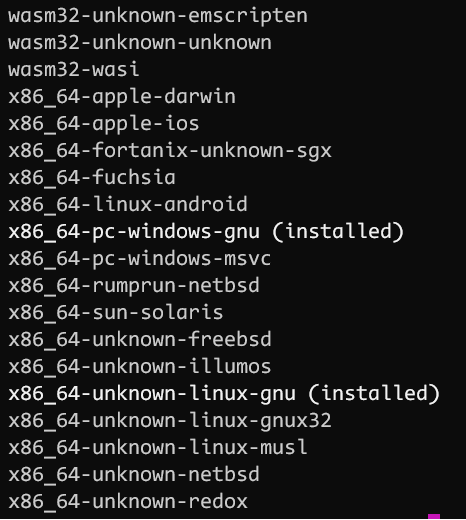
\includegraphics[scale=0.5]{rust_target.png}
  \caption{Rust支持的目标文件架构}
  \label{fig:rust_target}
\end{figure}

需要编译对应架构的目标文件,则需要添加对应架构的工具链
\begin{code-block}{bash}
# 针对ARM V7架构的工具链
rustup target add armv7-unknown-linux-gnueabihf
# 针对ARM X64架构的工具链
rustup target add aarch64-unknown-linux-gnu
# 针对Windows 64的工具链
rustup target add x86_64-pc-windows-gnu
\end{code-block}

除了添加工具链之外,还需要安装对应的交叉编译工具
\begin{code-block}{bash}
# 针对Windows 64的交叉编译工具
dnf install mingw64-gcc mingw64-winpthreads-static -y
\end{code-block}

而针对ARM V7以及ARM X64的交叉编译工具,则是使用gcc-linaro工具链即可。

针对Windows 64的交叉编译方法比较简单,其编译指令如下:
\begin{code-block}{bash}
cargo build --release --target=x86_64-pc-windows-gnu
\end{code-block}

针对ARM V7和ARM X64的编译过程稍微复杂一些,其操作如下:
\begin{enumerate}
  \item 创建配置文件:进入rust工程的根目录
\begin{mdframed}[topline=false, bottomline=false, leftline=false,
    rightline=false, backgroundcolor=lbcolor]
\begin{minted}[fontsize=\scriptsize,linenos=false,breaklines=true,
    breakanywhere,breaksymbolleft=,breakanywheresymbolpre=,]{bash}
mkdir .cargo
touch .cargo/config
\end{minted}
\end{mdframed}

  \item 修改配置文件,设置交叉编译工具
\begin{mdframed}[topline=false, bottomline=false, leftline=false,
    rightline=false, backgroundcolor=lbcolor]
\begin{minted}[fontsize=\scriptsize,linenos=false,breaklines=true,
    breakanywhere,breaksymbolleft=,breakanywheresymbolpre=,]{bash}
cat >.cargo/config<<EOF
[target.armv7-unknown-linux-gnueabihf]
linker = "/opt/gcc-linaro-7.5.0-2019.12-x86_64_arm-linux-gnueabihf/bin/arm-linux-gnueabihf-gcc"
ar = "/opt/gcc-linaro-7.5.0-2019.12-x86_64_arm-linux-gnueabihf/bin/arm-linux-gnueabihf-ar"

[target.aarch64-unknown-linux-gnu]
linker = "/opt/gcc-linaro-7.5.0-2019.12-x86_64_aarch64-linux-gnu/bin/aarch64-linux-gnu-gcc"
ar = "/opt/gcc-linaro-7.5.0-2019.12-x86_64_aarch64-linux-gnu/bin/aarch64-linux-gnu-ar"

EOF
\end{minted}
\end{mdframed}

  \item 进行交叉编译:
\begin{mdframed}[topline=false, bottomline=false, leftline=false,
    rightline=false, backgroundcolor=lbcolor]
\begin{minted}[fontsize=\scriptsize,linenos=false,breaklines=true,
    breakanywhere,breaksymbolleft=,breakanywheresymbolpre=,]{bash}
# 针对ARM V7(32位)
cargo build --release --target=armv7-unknown-linux-gnueabihf
# 针对ARM X64
cargo build --release --target=aarch64-unknown-linux-gnu
\end{minted}
\end{mdframed}

\end{enumerate}

\section{Rust的控制流}
Rust的控制流和其他语言相同,都包含了判断和循环。Rust的判断流通过if/else以及
else if实现,但是并不包含switch语句。当if-else的结构过多,则会导致代码比较
杂乱,因此Rust还提供了另外一种语法格式:match来解决这些问题。

Rust的if/else可以用在普通的判断场景,但判断条件必须是bool类型的数据,不允许
使用其他类型作为判断的依据,所以,下列的代码是错误的:
\begin{code-block}{rust}
let a = 10;

// error, a is not a boolean type
if a {
    ...
}
\end{code-block}

Rust也有自己的3元运算符,其使用基本如下:
\begin{code-block}{rust}
let a = 100;
let b = 200;
let number = if a > b {
    b
} else {
    a
};

\end{code-block}

Rust的循环操作比较丰富,除了常见的for,while之外,还提供了loop循环。默认情况
下,loop语句是无限循环。
\begin{code-block}{rust}
loop {
    println!("Forever loop");
}
\end{code-block}
通常情况下,loop是和break配合使用的。和其他语言不太一样,在其他语言当中,break
关键字只是用于中断当前运行的循环,但是Rust当中,break可以后接表达式,将退出
的信息返回给调用者,如下:
\begin{code-block}{rust}

let mut counter = 0;

loop {
    println!("loop");
    if counter > 10 {
        break;
    }
    counter += 1;
}

counter = 0;

let result = loop {
    counter += 1;
    if 10 == counter {
        break counter * 2;
    }
};
\end{code-block}
当上述循环退出之后,result的值就相当于counter的2倍。

而其他语言当中常用的while/for循环,Rust也同样支持,但是,不支持do-while结构。
相比较而言,Rust的while是最简单的,其示例如下:
\begin{code-block}{rust}
let mut number = 3;

while number != 0 {
    println!("{}!", number);
    number = number - 1;
}
\end{code-block}
实际使用当中,for循环使用比较多。Rust的for循环和python类似,都是for-in结构。
具体的示例如下:
\begin{code-block}{rust}
let array = [1, 2, 3, 4, 5];

// 引用权
for element in &array {
    println!("The value is {ele}", ele = element);
}

for element in array.iter() {
    println!("The value is {ele}", ele = element);
}

// 取值范围为[1..10),rev表示反序输出
for ele in (1..10).rev() {
    println!("The element is {ele}", ele = ele);
}

// 取值范围为[1..10]
for ele in (1..=10).rev() {
    println!("The element is {ele}", ele = ele);
}
\end{code-block}

\section{所有权与slice}
Rust当中没有垃圾回收机制,因此,不存在“万恶的GC时间”。但是,Rust采用了所有权
这一特点来解决垃圾回收的问题。对于同一个对象(符合数据类型),同一时间只有一个变量可以持有其
所有权,其他的变量无法使用。
\begin{code-block}{rust}
let a = String::from("hello");
let b = a; // a对象被转移给b,相当于a所代指的内存内容被转移给了b变量,a被清空

// a对象在此之后无法使用,已经被回收
// 如果还需要让a可以被继续使用,则上述操作应当变更为如下
/*
let a = String::from("hello");
let b = a.clone();
*/
\end{code-block}
为了能够同时使用多个变量对同一个对象进行操作和运算,Rust使用引用和切片来解决
这个问题。
\begin{code-block}{rust}
let a = String::from("hello");
let b = &a;

// a对象还可以继续使用
\end{code-block}

对于数组类型的引用操作,通常使用切片操作来实现。Rust的切片和Python当中的相同,
只是缺少了反向切片和负数切片。常见的切片类型,或者说经常使用切片操作的,就是
字符串String。字符串的切片类型是\&str,字符串操作函数通常的都是使用字符串切片
实现的,如下:
\begin{code-block}{rust}
fn main() {
    let my_string = String::from("hello world");
    let my_string_literal = "hello world";

    let copy_1 = first_word(&my_string[..]);
    let copy_2 = first_word(&my_string_literal);
    let copy_3 = first_word(my_string_literal);
}

fn first_word(s: &str) -> &str {
    return &s[..];
}
\end{code-block}
需要注意,字符串的字面量,实际就是字符串切片数据类型。

\section{数据类型}
Rust当中的数组稍微有些特殊,在定义的时候,可以指定数据类型和长度,也可以进行
自动推导,还可以使用简便定义的方式。其基本使用如下:
\begin{code-block}{rust}
// the same as let array: [u32; 5] = [1,2,3,4,5];
let array = [1, 2, 3, 4, 5];
// the same as let a = [3,3,3,3,3]
let a = [3; 5];
\end{code-block}

数组作为函数参数时,长度必须作为数组的一部分进行传递:
\begin{code-block}{rust}
fn show_array(array: [u32; 5]) {
    ...
}
\end{code-block}

数组元素的迭代可以使用两种方式:1种是直接迭代,一种是使用iter函数进行:
\begin{code-block}{rust}
for item in array.iter() {
    println!("{}", item);
}

for item in &array {
    println!("{}", item);
}
\end{code-block}
但是,数组是无法迭代的,能够直接迭代的是切片(slice),而数组的引用就是一个
slice。同样的,切片也是可以进行迭代的,如下示例:
\begin{code-block}{rust}
fn show_array(array: &[u32; 5]) {
    for item in array.iter() {
        println!("{}", item);
    }

    for item in array {
        println!("{}", item);
    }
}
\end{code-block}

同C++相同,Rust也提供了Vector数据类型,其基本的用法和C++类似:
\begin{code-block}{rust}
// 初始化空的vector
let mut v: Vec<i32> = Vec::new();
// 自动推导生成vector
let v1 = vec![1, 2, 3];
\end{code-block}

Vector默认只能存放相同类型的数据,无法存放不同的数据类型。如果遇到了需要存放
不同的数据类型,则通常使用vector+enum的方式进行实现:
\begin{code-block}{rust}
let ips = vec![
    IPADDR::V4(255, 255, 255, 254),
    IPADDR::V6(String::from("fe80::708f:7183:c02b:1758")),
];
\end{code-block}

Vector数据需要注意的是遍历操作。默认情况下,使用for-in结构对vector进行遍历
操作,操作的是vector的值,并不是vector的引用,所以,一旦遍历结束,则该vector
就无效了。如果并不是需要只对vector进行遍历,后续还有其他操作,则在遍历的时候,
一定要采用引用,如下:
\begin{code-block}{rust}
for ele in &ips {
    println!("{}", ele);
}
\end{code-block}

字符串是常用的数据类型,针对字符串,也有一些需要注意。默认的情况下,所有的
字符串字面量都是切片,不是字符串变量,但是可以转换成字符串:
\begin{code-block}{rust}
let s = String::from("char");
let r = "char".to_string();
\end{code-block}

字符串的拼接与Python类似,但是需要注意有略微的不同:
\begin{code-block}{rust}
let s1 = String::from("Hello, ");
let s2 = String::from("world!");
let s3 = s1 + &s2; // 注意 s1 被移动了,不能继续使用
\end{code-block}

如果需要多次执行字符串的拼接,则最好使用format操作:
\begin{code-block}{rust}
let s1 = String::from("tic");
let s2 = String::from("tac");
let s3 = String::from("toe");

let s = format!("{}-{}-{}", s1, s2, s3);
\end{code-block}

字符串在Rust当中的本质是是一个 Vec<u8> 的封装,可以按照unicode的方式(字符)
进行处理,也可以按照原始字节(u8数据)的方式进行处理。
\begin{code-block}{rust}
// 按照字符类型处理
for c in "helllo".chars() {
    ...
}

// 按照字节进行处理
for b in "hello".bytes() {
    ... // 如果进行输出,则输出的都是223,123等类似的数字数据
}
\end{code-block}

Map(映射)是Rust的另外一种容器数据类型,和Python的字典很像,但是,Rust的map
的键只能是同种类型的,值也只能是同种类型的,无法像Python的字典一样的灵活。常
用的map主要是HashMap和BTreeMap。构建map数据可以使用new,也可以使用collect方法:
\begin{code-block}{rust}
use std::collections::HashMap;

let mut scores = HashMap::new();

scores.insert(String::from("Blue"), 10);
scores.insert(String::from("Yellow"), 50);

let teams  = vec![String::from("Blue"), String::from("Yellow")];
let initial_scores = vec![10, 50];

// 将其他的类型组合成map
// HashMap<_, _> 类型注解是必要的,因为可能 collect 很多不同的数据结构,
// 而除非显式指定否则 Rust 无从得知你需要的类型。但是对于键和值的类型参数来说,
// 可以使用下划线占位,而 Rust 能够根据 vector 中数据的类型推断出 HashMap 所包含的类型
let scores1: HashMap<_, _> = teams.iter().zip(initial_scores.iter()).collect();
\end{code-block}

Map数据类型对于普通的数值类型数据,不会获取其所有权,但是,对于复合数据类型包括
String,都会获得相关的所有权,如下:
\begin{code-block}{rust}
let field_name = String::from("Favorite color");
let field_value = String::from("Blue");

let mut map = HashMap::new();
map.insert(field_name, field_value);
// 在此之后,field_name和field_value无法再被访问和使用。
\end{code-block}

Map元素的获取,可以直接采用[]进行,也可以采用get的方式:
\begin{code-block}{rust}
let team_name = String::from("Blue");
let score_num = scores[&team_name]
let score = scores.get(&team_name);
\end{code-block}
但需要注意,上述代码当中,score的类型为Some(T),需要按照枚举Option的方式进行处理。

Map的迭代同样需要使用for-in循环,并且需要注意所有权的使用:
\begin{code-block}{rust}
for (key, value) in &scores {
    println!("{}: {}", key, value);
}
\end{code-block}

和Python有区别的是,Rust允许这样的一种操作:当只有map当中键不存在时,才进行插入,
否则什么也不做:
\begin{code-block}{rust}
scores.entry(String::from("Yellow")).or_insert(50);
scores.entry(String::from("Blue")).or_insert(50);
\end{code-block}

\section{复杂数据类型}
\subsection{结构体}
Rust的结构体和Golang的结构体非常类似,直接使用struct关键字进行定义。
\begin{code-block}{rust}
struct User {
    username: String,
    age: u8,
    email: String,
    activate: bool,
}
\end{code-block}
结构体的初始化操作也类似Golang,如下:
\begin{code-block}{rust}
let user = User {
    username: String::from("zhangjl"),
    age: 32,
    email: String::from("zhangjl@awcloud.com"),
    activate: true,
};
\end{code-block}
如果已经有一个结构体实例,可以直接从已有的实例当中继承部分的属性:
\begin{code-block}{rust}
let user = User {
    username: String::from("zhangjl"),
    email: String::from("zhangjl@awcloud.com"),
    ..user
};
\end{code-block}

上述的结构体,由于每个字段都有名称,可以称之为命名结构体,而Rust当中,也支持
没有字段名称的结构体,称之为无名结构体,或者匿名结构体。这种类型的结构体,通
常是类似于元组的形式,如下:
\begin{code-block}{rust}
struct Color(u8, u8, u8);

fn show_color(color: &Color) {
    println!(
        "The RGB value is R:{}, G:{}, B:{}",
        color.0, color.1, color.2
    );
}
\end{code-block}
同样的,Rust也存在一种特殊的结构体:空结构,其形式基本如下:
\begin{code-block}{rust}
struct Empty();
\end{code-block}

Rust当中的struct实际和C++/Java当中的类(class)非常类似,都是对象类型,必然
有属于自己的函数(方法)。通常的,Rust的struct的函数需要使用impl关键字进行
定义和实现,其示例如下:
\begin{code-block}{rust}
impl User {
    fn show(&self) {
        println!(
            "The user info is: Name: {}, Age: {}, email: {}, and activate: {}",
            self.username, self.age, self.email, self.activate
        );
    }
    fn create() -> User {
        return User {
            username: String::from(""),
            age: 0,
            email: String::from(""),
            activate: false,
        };
    }
}
\end{code-block}
上述例子当中,show是结构体User的方法(method),可以直接使用User的实例进行调
用,而create则是一个独特的函数,表示隶属于User这个结构体,需要使用作用域符号
::进行调用,类似于C++/Java当中的构造函数,在Rust当中称之为关联函数。使用示例
如下所示:
\begin{code-block}{rust}
let new_user = User::create();
new_user.show();
\end{code-block}

\subsection{枚举与match}
Rust当中的枚举类型相当强大,和C/C++当中的枚举不一样,Rust的枚举元素可以是任意
类型,甚至可以类似于结构体,拥有自己的方法。普通的枚举定义方式如下:
\begin{code-block}{rust}
enum IpAddrKind {
    V4,
    V6,
}
\end{code-block}
通常情况下,枚举的使用也很简单,如下示例:
\begin{code-block}{rust}
let four = IpAddrKind::V4;
let six = IpAddrKind::V6;
\end{code-block}
这样的使用,与C/C++当中的枚举使用方式基本一致,只是用于作为标志量进行传递。

如果需要根据枚举的元素进行相关的数值转换或者获取,则需要使用match进行操作,
如下:
\begin{code-block}{rust}
enum Coin {
    Penny,
    Nickel,
    Dime,
    Quarter,
}

fn value_in_cents(coin: Coin) -> u8 {
    match coin {
        Coin::Penny => 1,
        Coin::Nickel => 5,
        Coin::Dime => 10,
        Coin::Quarter => 25,
    }
}
\end{code-block}

在Rust当中,还有更为高级的用法,将枚举作为特殊的结构体,同样的,枚举类型也
可以拥有自己的方法,关联方法以及特殊的格式化输出方法等等。
\begin{code-block}{rust}
use std::fmt;

enum IPADDR {
    V4(u8, u8, u8, u8),
    V6(String),
}

impl IPADDR {
    fn show(&self) {
        match self {
            IPADDR::V4(a, b, c, d) => println!(
                "This is the ipv4 addr {}.{}.{}.{}", a, b, c, d),
            IPADDR::V6(v6) => println!("The V6 addr is ipv6 addr {}", v6),
        }
    }

    fn format(&self) -> String {
        match self {
            IPADDR::V4(a, b, c, d) => {
                let _v4 = format!("{}.{}.{}.{}", a, b, c, d);
                _v4
            }
            IPADDR::V6(v6) => v6.to_string(),
        }
    }
}

impl fmt::Display for IPADDR {
    fn fmt(&self, f: &mut fmt::Formatter) -> fmt::Result {
        match self {
            IPADDR::V4(a, b, c, d) => write!(f, "{}.{}.{}.{}", a, b, c, d),
            IPADDR::V6(v6) => write!(f, "{}", v6.to_string()),
        }
    }
}
\end{code-block}
在使用复杂的枚举类型时,match是一个非常
重要的操作。使用这种类型的枚举时,如同普通的struct一样的使用:
\begin{code-block}{rust}
let addr = IPADDR::V4(127, 0, 0, 1);
let addr_v6 = IPADDR::V6(String::from("fe80::708f:7183:c02b:1758"));

addr.show();
addr_v6.show();
println!("{}", addr);
\end{code-block}

Rust的枚举类型可以嵌套各种其他的类型,包括枚举类型本身。一个设计良好的枚举
类型通常可能包括了各种数据类型:
\begin{code-block}{rust}
enum Message {
    Quit, // 没有包含任何数据类型,相当于空结构体
    Move { x: i32, y: i32 }, // 匿名结构体
    Write(String), // 类元组结构体
    ChangeColor(i32, i32, i32), // 类元组结构体
}

impl Message {
    fn call(&self) {
        match self {
            Message::Quit => println!("Received the quit signal, exiting..."),
            Message::Move { x, y } => println!("Move a to {}, {}", x, y),
            Message::Write(_str) => println!("Write message {}", _str),
            Message::ChangeColor(a, b, c) => println!("Change the color to {}, {}, {}", a, b, c),
        }
    }
}
\end{code-block}
上述枚举类型的使用示例如下:
\begin{code-block}{rust}
let mut msg = Message::Quit;
msg.call();

msg = Message::Move { x: 100, y: 200 };
msg.call();

msg = Message::Write(String::from("zhangjl"));
msg.call();

msg = Message::ChangeColor(255, 0, 0);
msg.call();
\end{code-block}

除了这些常规的和自定义的枚举类型之外,Rust还提供了一个非常常用的特殊枚举类型:
Option。Option的实际实现非常简单:
\begin{code-block}{rust}
enum Option<T> {
    Some(T),
    None,
}
\end{code-block}
Option通常和Some、None、match一起使用。需要说明的是,Rust当中并没有普通意义上
的NULL或者None,无法像C/C++一样,将NULL或者None赋值给指针,因为Rust当中没有
指针的概念。None在Rust当中,同样表示空,但是,是作为Option的一种有效的数据
形式使用。Option的使用如下:
\begin{code-block}{rust}
let x: Option<i8> = None
let y: Option<i8> = Some(5);
\end{code-block}
注意,Some数据类型无法直接和其他的数据类型进行直接的计算,必须进行拆包才可
正常使用,其使用示例如下:
\begin{code-block}{rust}
fn plus(x: Option<u8>) -> Option<u8> {
    match x {
       None => None,
       Some(i) => Some(i + 1),
    }
}

let six = plus(Some(5));
let six_num = six.unwrap();

let none_type = plus(None);
let none_value = none_type.unwrap_or_default();
\end{code-block}

Match可以匹配多个条件,但是,如果只需要匹配个别的情况,即需要忽略一些情况,则
需要使用通配符进行处理,通配符为\_,其基本使用如下:
\begin{code-block}{rust}
let some_u8_value = 0u8;
match some_u8_value {
    1 => println!("one"),
    3 => println!("three"),
    5 => println!("five"),
    7 => println!("seven"),
    _ => (),
}
\end{code-block}
如果本身的情况很少,只需要考虑2种情况,使用match则显得比较罗嗦,可以使用if-let
结构,该结构使用示例如下:
\begin{code-block}{rust}
if let Some(3) = some_u8_value {
    println!("three");
}

let mut count = 0;
if let Coin::Quarter(state) = coin {
    println!("State quarter from {:?}!", state);
} else {
    count += 1;
}
\end{code-block}

同样的,match也可以和其他的数据类型一起使用:
\begin{code-block}{rust}
let v = vec![1, 2, 3];
// 从集合vector当中获取索引标记的数据
let ele = match v.get(1) {
    // Some(&ref),即some当中的参数永远是引用数据类型
    Some(val) => *val,
    None => 0,
};
println!("{}", ele);
\end{code-block}

\section{包/模块管理}
在大型项目当中,Rust同样提供了代码的管理机制。和Python、Golang等不同,Rust的
代码管理可以分为包(crate)和模块(mod)。这2种模式有不少的区别。Mod模式类似
于Python的管理方式,而crate则是另外一种管理方式。这2种方式可以相互嵌套使用。
在使用这2种方式之前,需要知道一个概念:Rust的路径寻找永远是从最顶层开始,即
与Cargo.toml同级的src下开始。Src路径,被称之为crate路径,即根路径。一切从crate
开始的路径,都称之为绝对路径;其他的方式,则称之为相对路径。

\subsection{Mod管理模式}
Mod管理模式和Python/Golang的路径管理类似,直接从当前工程的src路径一直往下进行
查找,直到最终找到。首先看一个Rust工程结构, 如下图\nameref{fig:rust_mod}所示。
\begin{figure}[H]
  \centering
  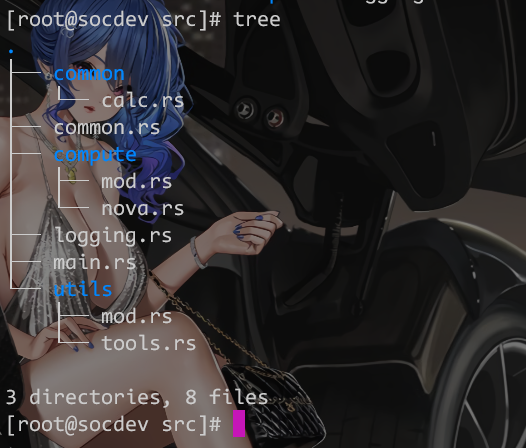
\includegraphics[scale=0.8]{rust_mod.png}
  \caption{Mod管理模式}
  \label{fig:rust_mod}
\end{figure}
其中,有几个特点:
\begin{enumerate}
  \item 从文件层次结构上,logging.rs、main.rs、common.rs、common、compute和
utils为同一层级,但是只有 main属于crate,其他都是属于crate管辖的范围,即在
逻辑上,logging.rs、compute、utils、common和common.rs属于main的下级模块
  \item compute和utils无法直接使用,只能使用这2个目录下的模块(文件)
\end{enumerate}

如果logging模块不需要使用其他模块,则内部无需特别的处理,其代码如下:
\begin{code-block}{rust}
pub fn logging() {
    println!("This is the logging function");
}
\end{code-block}
由于main属于crate,logging归属crate管理,相当于是logging是main的子模块,因此
在main当中,只能使用相对路径访问logging,不能使用crate的绝对路径,其使用方式
如下:
\begin{code-block}{rust}
mod logging;

use logging as log; // 模块别名
\end{code-block}
在使用模块的时候,一定注意,mod关键字必须放在use之前。而common和logging属于
相同的层次,如果在common当中需要使用logging模块,则必须使用全路径crate。如果
如同在main当中使用logging一样
\begin{code-block}{rust}
// common.rs
mod logging;
// mod crate::logging; 同样是错误的代码
\end{code-block}
则会出现下列错误:
\begin{figure}[H]
  \centering
  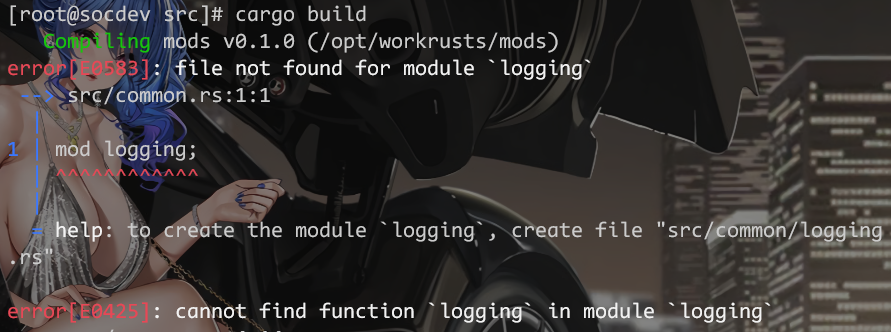
\includegraphics[width=\linewidth]{rust_mod_error1.png}
  \caption{模块错误1}
  \label{fig:rust_mod_error1}
\end{figure}
而正确的使用方式(全路径)则如下:
\begin{code-block}{rust}
// common.rs
use crate::logging;
...
\end{code-block}

如果强行需要在common.rs文件当中,以相对路径的方式使用logging,则必须将logging.rs
模块放到common当中,即按照上述的错误提示,将logging作为common的一个子模块。
只有父模块可以通过相对路径的方式访问子模块,平级模块之间,或者没有亲缘关系
的模块之间,只能通过绝对路径的方式使用。

在上述的代码当中,有一个比较奇怪的现象:同时存在common和common.rs。这是Rust
管理的一种模式。默认情况下,Rust的模块有2种模式:文件形式和文件夹形式。

文件夹形式实际上就是将一个文件夹作为Rust的模块进行使用。通常情况下,文件夹
模式的模块形式如下:
\begin{figure}[H]
  \centering
  
\includegraphics[scale=0.5]{rust_mod_directory.png}
  \caption{文件夹模块}
  \label{fig:rust_mod_directory}
\end{figure}
其中,nova.rs当中的内容和普通的Rust文件类似,基本如下:
\begin{code-block}{rust}
// nova.rs
pub fn nova() {
    println!("This is the nova function");
}
\end{code-block}
重点是mod.rs这个文件。该文件实际上是用于定义/暴露compute这个文件夹当中的模块。
如果compute文件夹缺少mod.rs,则compute无法被识别成一个合法的Rust模块,即无法
使用compute当中的任何代码。而mod.rs的内容比较特殊,和nova.rs的内容并不一致,
其内容大致如下:
\begin{code-block}{rust}
// mod.rs
pub mod nova;
pub mod driver;
\end{code-block}
通过上述的代码,将nova.rs作为一个可供外部使用模块。同样的,由于nova.rs和
drvier.rs属于同级目录,如果需要在nova.rs当中使用driver.rs所提供的功能,则
需要使用绝对路径的方式对其进行引用:
\begin{code-block}{rust}
// nova.rs
use crate::compute::driver;
...
\end{code-block}

同名文件和文件夹的模式,则是另外一种模块的管理方法。这种管理方式,其文件组织
形式如下:
\begin{figure}[H]
  \centering
  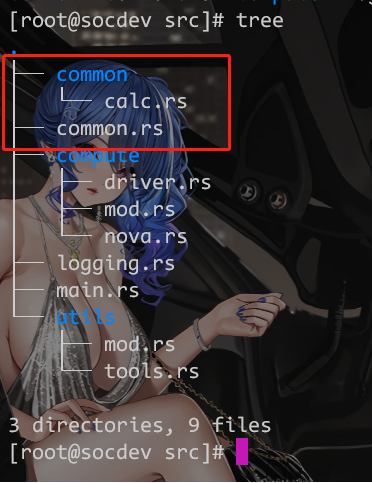
\includegraphics[scale=0.3]{rust_mod_file.png}
  \caption{同名文件形式}
  \label{fig:rust_mod_file}
\end{figure}
在这种模式下,calc.rs的内容和普通的相同,而重点在于外部的common.rs。该文件的
功能实际上和上述所说的mod.rs类似,都是用于暴露模块的。该文件的内容大致如下:
\begin{code-block}{rust}
// common.rs
pub mod calc; // 将calc.rs当中的内容进行导出

use crate::logging;

fn common() {
    logging::logging();
}
\end{code-block}

将上述的概念和技术进行整合,整体的工程文件内容大致如下:
\begin{code-block}{rust}
// common.rs
pub mod calc;

use crate::logging;

fn common() {
    logging::logging();
}

// common/calc.rs
pub fn add() {
    println!("This is the add function");
}

// compute/driver.rs
pub fn call() {
    println!("This is the driver::call function");
}

// compute/nova.rs
use crate::compute::driver;
use crate::logging;
use crate::utils::tools;

pub fn nova() {
    println!("This is the nova function");
}

pub fn use_parent() {
    println!("Use the logging function in child mod");
    logging::logging();
}

pub fn use_other() {
    println!("Use the logging function in child mod");
    tools::execute();
}

pub fn deive() {
    driver::call();
}

// compute/mod.rs
pub mod driver;
pub mod nova;

// logging.rs
pub fn logging() {
    println!("This is the logging function");
}

// utils/tools.rs
use crate::logging as log;

pub fn execute() {
    println!("This is the execute function");
    log::logging();
}

pub mod tools;

// main.rs
mod common;
mod compute;
mod logging;
mod utils;

use common as com;
use compute::nova;
use logging as log;
use utils::tools;

fn main() {
    log::logging();
    nova::nova();
    nova::use_other();
    nova::use_parent();

    tools::execute();
    com::calc::add();
}
\end{code-block}

\subsection{Crate管理模式}
Crate管理模式通常用于在自己的Rust代码当中引用别人的代码或者类库。和Python以及
Golang的直接import方式不同,Rust的mod模式并不能直接使用别人的代码(除了标准库),
只能通过Crate的方式。Crate方式可以管理其他人的公开代码,也可以管理自己编写的
类库代码。

\subsubsection{使用第三方代码}
一般方式下,需要修改Rust工程的Cargo.toml文件,在dependencies段当中加入需要使用
的类库名称,如下:
\begin{code-block}{toml}
[dependencies]
regex = "0.1.41"
\end{code-block}
然后,在自己的代码当中添加如下的语句:
\begin{code-block}{rust}
use regex::Regex;

fn main() {
    let re = Regex::new(r"^\d{4}-\d{2}-\d{2}$").unwrap();
    println!("Did our date match? {}", re.is_match("2014-01-01"));
}
\end{code-block}
运行cargo build指令时,会直接从cargo.io进行下载。

如果需要使用的依赖库并不在cargo.io,而是放在了类似于github等地方,也可以修改
Cargo.toml文件,类似如下:
\begin{code-block}{toml}
[dependencies]
# 可以和包不同名,也可以同名
my_rust_lib_1={package="my_lib_1",git="ssh://git@github.com/lpxxn/my_rust_lib_1.git",tag="v0.0.2"}
my_rust_lib_2={package="my_lib_1",git="https://github.com/lpxxn/my_rust_lib_2.git",branch="master"}
\end{code-block}
运行cargo build指令时,同样会去github等代码管理仓库下载指定的依赖代码。

Crate模式不仅可以管理外部第三方依赖代码,同样可以用于管理本地的代码。

\subsubsection{Crate管理本地代码}
在使用这种方式之前,先了解一下crate的一些概念。
\begin{itemize}
  \item 包是cargo的一个功能,当执行cargo new xxxx的时候就是创建了一个包。
  \item crate是二进制或者库项目。rust约定在Cargo.toml的同级目录下包含src目录
并且包含main.rs文件,就是与包同名的二进制crate,如果包目录中包含src/lib.rs,
就是与包同名的库crate
  \item 包内可以有多crate,多个crates就是一个模块的树形结构
  \item 如果一个包内同时包含src/main.rs和src/lib.rs,那么他就有两个crate,
如果想有多个二进制crate,rust约定需要将文件放在src/bin目录下,每个文件就是
一个单独的crate
  \item crate根用来描述如何构建crate的文件。比如src/main.rs或者src/lib.rs就
是crate根。crate根文件将由Cargo传递给rustc来实际构建库或者二进制项目
  \item 带有Cargo.toml文件的包用来描述如何构建crate,一个包可以最多有一个库
crate,任意多个二进制crate。
\end{itemize}

包含多个二进制crate的Rust项目大致如下:
\begin{figure}[H]
  \centering
  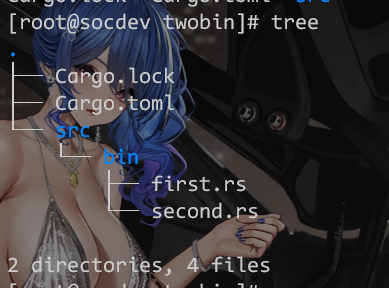
\includegraphics[scale=0.5]{rust_more_bin.png}
  \caption{多个二进制}
  \label{fig:rust_more_bin}
\end{figure}
对这个项目进行编译,将会得到2个二进制文件:first和second,而不再是之前的和
根路径同名,得到的结果类似下面:
\begin{figure}[H]
  \centering
  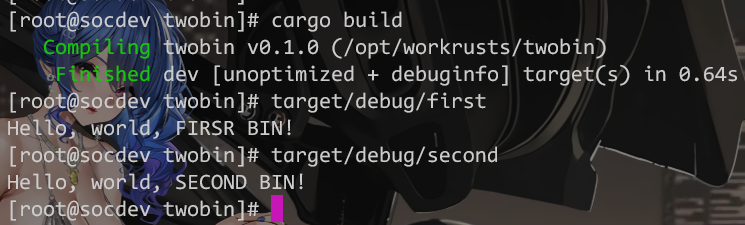
\includegraphics[width=\linewidth]{rust_more_bin_res.png}
  \caption{多个二进制编译结果}
  \label{fig:rust_more_bin_res}
\end{figure}

创建一个包含lib的Rust项目,则稍微有些区别,首先创建一个二进制的crate:
\begin{code-block}{bash}
cargo new projects
\end{code-block}
然后,在这个二进制的crate当中,创建一个lib:
\begin{code-block}{bash}
cd projects
cargo new --lib first
\end{code-block}
同样的,可以在这个二进制的crate当中,创建多个lib,最后的文件结构大致如下:
\begin{figure}[H]
  \centering
  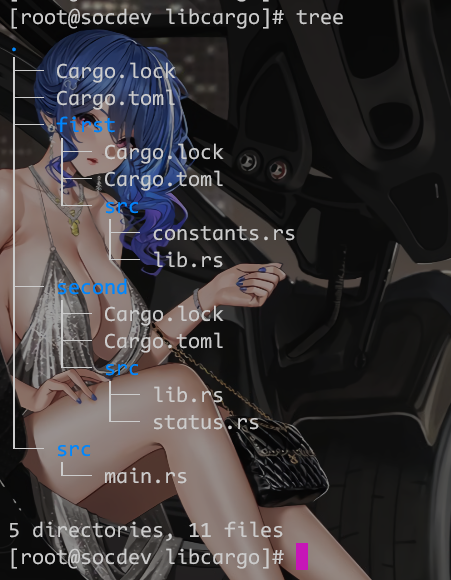
\includegraphics[scale=0.6]{rust_lib.png}
  \caption{Lib形式的crate}
  \label{fig:rust_lib}
\end{figure}

到目前为止,src当中的代码是无法使用first和second当中的代码的,而且,first和
second这2个路径当中的代码,也并不是合法并可用的Rust lib库。首先需要解决的,
就是使得first和second成为合法的Rust lib库。在first和second这2个文件夹当中,
不再拥有mod.rs,取而代之的则是lib.rs,需要在lib.rs的同级或者下级目录,添加
合法的rs文件,然后,在lib.rs使用pub对这些模块进行导出。以first这个lib为例,
其src目录下的文件,内容应当大致如下:
\begin{code-block}{rust}
// constants.rs
pub enum VERSION {
    V4,
    V6,
}

// lib.rs
pub mod constants;
\end{code-block}

经过以上的改写之后,first便成为了一个合法可用的Rust lib库。如果需要在顶层的
main.rs当中使用这个lib库,还需要修改顶层Cargo.toml的内容,将first作为二进制
crate的依赖:
\begin{code-block}{toml}
[dependencies]
# path表示lib库的路径,version则是lib库的Cargo.toml当中所包含的version
first = { path = "first", version = "0.1.0" }
second = { path = "second", version = "0.1.0" }
\end{code-block}

通过上述的修改,则可以在二进制crate当中,使用first和second这2个lib库了。
\begin{code-block}{rust}
use first::constants;
use second::status;
\end{code-block}

有的时候,为了更加清晰的描述当前的crate与其他crate的关系,可以直接使用extern
进行标记:
\begin{code-block}{rust}
extern crate first;
extern crate second;

use first::constants;
use second::status;
\end{code-block}

如果lib之间存在依赖关系,同样可以在lib的Cargo.toml当中添加相关的依赖关系。
比如,假设second依赖于first模块,则可以在second的Cargo.toml当中添加如下内容:
\begin{code-block}{toml}
[dependencies]
first = { path = "../first", version = "0.1.0" }
\end{code-block}

然后,直接在second的代码当中使用first的内容即可。同样的,在second当中使用first
的内容,可以参考下面的案例:
\begin{code-block}{rust}
extern crate first;
use first;

...
\end{code-block}

相比于mod模式,crate模式更加清晰一些。

\subsection{大规模的管理方式——workspace}
上述的2种模块管理方式,解决了路径查找的问题。但是,如果是针对大型项目,特别是
代码量类似于OpenStack这种规模的,mod和crate模式都有些难以管理。这时,就需要
使用workspace的方式进行管理。Workspaces的方式,实际上是对mod和crate的综合和
高层次总结,其使用方式大致如下:

\begin{outline}[enumerate]
\1 创建工作目录
\begin{code-in-enumerate}{bash}
mkdir works
\end{code-in-enumerate}

\1 创建需要的crate
\begin{code-in-enumerate}{bash}
cargo new first --bin
cargo new second --bin
cargo new shared --lib
\end{code-in-enumerate}

\1 创建工作管理的Cargo.toml文件
\begin{code-in-enumerate}{bash}
cat >Cargo.toml<<EOF
[workspace]
members = [
    "first",
    "second",
    "shared",
]
EOF
\end{code-in-enumerate}

\1 编译所有的crate
\begin{code-in-enumerate}{bash}
cargo build
# 或者
# cargo build --workspace
\end{code-in-enumerate}

\1 编译指定的bin crate
\begin{code-in-enumerate}{bash}
cargo build --bin first
\end{code-in-enumerate}

\1 编译指定的包
\begin{code-in-enumerate}{bash}
cargo build --package first
\end{code-in-enumerate}
\end{outline}

到目前为止,first和second为2个bin类型的crate,可以直接编译运行,而shared则是
一个lib库,并且,上述3个crate之间没有任何关联。如果first和second需要使用shared
当中的模块,则对应的,需要在first以及second目录下的Cargo.toml添加类似的如下
内容:
\begin{code-block}{toml}
[dependencies]
shared = { path = "../shared" , version = "0.1.0"}
\end{code-block}

然后修改second的main.rs如下即可:
\begin{code-block}{toml}
extern crate shared;
use shared::utils;

...
\end{code-block}
随后按照之前的方式进行编译和使用即可。

\subsection{模块管理的其他注意事项}

\begin{outline}[enumerate]
\1 提升命名空间

有的时候,Rust的代码层级非常深,比如下面:
\begin{code-in-enumerate}{rust}
pub mod english {
    pub mod greetings {
        pub fn hello() {
            println!("Hello!")
        }
        pub fn hey_guies() {
            println!("Hey, guies!")
        }
    }
}
\end{code-in-enumerate}
如果我们需要使用hello这个方法,则可能的方式多半如下:
\begin{code-in-enumerate}{rust}
english::greetings::hello();
\end{code-in-enumerate}
如果想将hello方法的访问缩短路径,则需要对代码进行改动:
\begin{code-in-enumerate}{rust}
// lib.rs
pub mod english {
    pub mod greetings {
        pub fn hello() {
            println!("Hello!")
        }
        pub fn hey_guies() {
            println!("Hey, guies!")
        }
    }
    // 将hello提升到english::hello
    pub use self::greetings::hello;
}

// 将hello提升到lib::hello
pub use english::greetings::hello;
\end{code-in-enumerate}
经过上述修改之后,使用的时候,可以按照下面的方式进行使用:
\begin{code-in-enumerate}{rust}
lib::chinese::hello(); // 对应pub use self::greetings::hello
lib::hello(); // 对应 pub use english::greetings::hello;
\end{code-in-enumerate}

\end{outline}

\section{格式化输出}
默认情况下,对于普通的数据类型(数值,字符,bool),Rust可以直接使用print语句
进行输出,但是,对于复合数据类型,比如自定义的结构体,数组等,直接使用print
则无法进行直接输出。为了直接输出这些数据,Rust提供了debug宏进行操作,允许直接
对复合数据类型进行格式化输出,如下所示:
\begin{code-block}{rust}
// 使用注解,启用debug特性,使之可以利用:?进行输出
#[derive(Debug)]
struct Rectangle {
    width: u32,
    height: u32,
}

fn main() {
    let rect1 = Rectangle { width: 30, height: 50 };

    println!("rect1 is {:?}", rect1);
}
\end{code-block}

但是debug的输出并不优雅,并且对于最终release版本的性能并不友好,因此,Rust
也提供了另外的机制,针对复合数据类型进行格式化输出——即Display。复合数据类型
需要实现一个Display方法,即可直接使用print语句进行输出。其示例如下:
\begin{code-block}{rust}
use std::fmt;

struct User {
    username: String,
    age: u8,
    email: String,
    activate: bool,
}

impl fmt::Display for User {
    fn fmt(&self, f: &mut fmt::Formatter) -> fmt::Result {
        write!(
            f,
            "Name:{}, Age: {}, Email: {}, Activate: {}",
            self.username, self.age, self.email, self.activate
        )
    }
}

...

fn main() {
    let new_user = User::create();
    println!("User: {}", new_user);
}
\end{code-block}

默认情况下,Rust提供了常用的格式化输出函数,主要有如下的几个:
\begin{enumerate}
  \item format!:将数据格式化成String对象
  \item print!:将数据格式化后输出到标准输出
  \item println!:类似print!,只是会追加换行操作
  \item eprint!:同print!,只是输出到标准的错误输出
  \item eprintln!:同eprint!,只是会追加换行操作
\end{enumerate}
常用的格式化输出函数,也用不同的用法,可以实现占位输出,命名输出,以及指定
数据宽度填充等等。具体使用如下:
\begin{code-block}{rust}
// 根据名称进行输出
println!(
    "The counter result is {counter} , and age is {age}",
    age = 100,
    counter = counter
);

// 根据位置进行输出
println!("{0}, {1}", "zhangjl", 18);

// 设置数据的显示宽度为6,向右对齐,不足的部分显示为空
// 同理,<则表示向左对齐
println!("{number:>width$}", number = 100, width = 6);
// 设置数据的显示宽度为6,向右对齐,不足的部分显示为0
println!("{number:>0width$}", number = 100, width = 6);
\end{code-block}
上述代码的执行结果大致如下图\nameref{fig:rust_format}所示。
\begin{figure}[H]
  \centering
  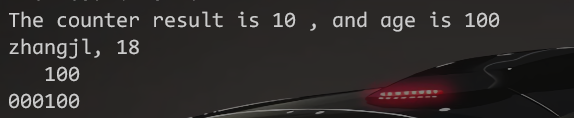
\includegraphics[scale=0.2]{rust_format.png}
  \caption{格式化输出}
  \label{fig:rust_format}
\end{figure}

\section{错误处理}
Rust的错误有多种,有可恢复的和不可恢复的。同样的,其处理机制也有多种,包含了panic
和Result模式。在默认的情况下,panic模式会打印程序的堆栈信息,并且清理堆栈数据,
最后退出,这样会造成生成的二进制程序比较大。如果需要二进制程序比较小,可以使用
abort终止堆栈信息的展开。比如,如果要禁止release模式的panic展开,可以修改Cargo.toml
文件如下:
\begin{code-block}{toml}
[profile.release]
panic = "abort"
\end{code-block}

如果需要展开所有的堆栈信息,则可如下进行操作:
\begin{code-block}{bash}
RUST_BACKTRACE=1 cargo run

// 全展开
RUST_BACKTRACE=full cargo run
\end{code-block}
则得到的效果可能如下:
\begin{figure}[H]
  \centering
  
\includegraphics[scale=0.2]{rust_err_panic_trace.png}
  \caption{错误堆栈}
  \label{fig:rust_err_panic_trace}
\end{figure}

通常而言,panic处理的错误都是不可恢复的,而如果是需要继续运行的,或者对应的错误
是可以进行处理的,则通常采用Result进行处理。Result是另外一个常用的enum类型,其定
义如下:
\begin{code-block}{rust}
enum Result<T, E> {
    Ok(T),
    Err(E),
}
\end{code-block}
其中,T和E都是泛型数据,而T表示正常运行时返回的数据,E表示返回的错误类型数据。

比如常见的打开文件操作,就可以使用Result进行错误处理:
\begin{code-block}{rust}
use std::fs::File;

fn main() {
    let f = File::open("hello.txt");

    let f = match f {
        Ok(file) => file,
        Err(error) => {
            panic!("Problem opening the file: {:?}", error)
        },
    };
}
\end{code-block}

错误是存在分类的,可以通过错误的类型,进行下一步的处理,比如,如果文件不存在,就
新建:
\begin{code-block}{rust}
use std::fs::File;
use std::io::ErrorKind;

fn main() {
    let fr = File::open("hello.txt");
    let f = match fr {
        Ok(file) => file,
        // 如果出现错误,就判断错误类型
        Err(error) => match error.kind() {
            // 如果错误类型是没有找到,就新建文件
            ErrorKind::NotFound => match File::create("hello.txt") {
                Ok(fc) => fc,
                Err(err) => panic!("{:?}", err),
            },
            // 其他错误。other可以替换成其他的任意字符。如果不想处理,则
            // _ => (),
            other => panic!("{:?}", other),
        },
    };
}
\end{code-block}

如果Match的分支过多,有可能导致代码逻辑比较复杂,难以理解。因此,Result也提供了
一种简化的方式,同样的,功能会相对较弱一些:
\begin{code-block}{rust}
use std::fs::File;

fn main() {
    // 如果文件不存在,则直接panic,并输出堆栈信息
    let fr = File::open("hello.txt").unwrap();
    // 如果文件不存在,则直接panic,但是,输出的是自定义(expect包含的)的错误信息
    let f = File::open("hello.txt").expect("Failed to open hello.txt");
}
\end{code-block}

如果不是在main函数当中出现错误,有的时候,实际上需要接收相关的错误,再进行处理,
则可以使用Result进行。再次强调,Result是一个泛型的枚举类型。
\begin{code-block}{rust}
use std::fs::File;
use std::io::{Error, ErrorKind, Read};

fn main() {
    match read_file() {
       Ok(s) => println!("The content of file is {}", s),
       Err(error) => panic!("{:?}", error),
    };

    // 或者使用变量进行接收
    let res = match read_file() {
        Ok(s) => s,
        Err(err) => {
            println!("ERROR:{:?}", err);
            "".to_string()
        }
    };
}

// 如果该函数执行成功,调用者会受到一个Ok(String),
// 否则,会接收到错误值
fn read_file() -> Result<String, Error> {
    let mut f = match File::open("Cargo.toml") {
        Ok(file) => file,
        Err(error) => return Err(error),
    };

    let mut s = String::new();
    let res = match f.read_to_string(&mut s) {
        Ok(_) => Ok(s),
        Err(err) => Err(err),
    };

    return res;
}
\end{code-block}

同样的,错误传递也可以进行简化,此时需要使用运算符?进行:
\begin{code-block}{rust}
fn read_file() -> Result<String, Error> {
    let mut f = File::open("hello.txt")?;
    let mut s = String::new();
    f.read_to_string(&mut s)?;
    Ok(s)
}
\end{code-block}
Result 值之后的?被定义为处理Result值的match表达式有着完全相同的工作方式。
如果Result的值是Ok,这个表达式将会返回Ok中的值而程序将继续执行。
如果值是Err,Err中的值将作为整个函数的返回值,就好像使用了return关键字一样,
这样错误值就被传播给了调用者。

?操作符大大简化了错误的处理流程,甚至于可以使用?进行链式调用,进一步简化代码:
\begin{code-block}{rust}
fn read_file() -> Result<String, Error> {
    let mut s = String::new();
    File::open("hello.txt")?.read_to_string(&mut s)?;
    Ok(s)
}
\end{code-block}

特别需要注意,?操作符只能用于返回类型为Result的函数当中,而main函数的返回类型是
(),不是Result,因此,直接在main函数当中使用?操作符则是错误的:
\begin{code-block}{rust}
fn main() {
    // 提示错误
    let f = File::open("hello.txt")?;
}
\end{code-block}

\section{泛型}
Rust当中使用<>操作符进行泛型的定义。泛型不仅可以用于函数和方法,也可以用于结构体。
\subsection{泛型结构体}
泛型结构体可以包含一种类型,也可以包含多种类型:
\begin{code-block}{rust}
struct Point<T> {
    x: T,
    y: T,
}
\end{code-block}
上述结构体由于只使用了一种类型T,因此x和y只能是相同的数据类型。如果要求x和y是不同
类型,则需要修改这个结构体的泛型定义:
\begin{code-block}{rust}
struct Point<T,U> {
    x: T,
    y: U,
}
\end{code-block}

泛型结构体的方法定义,则和之前的普通结构体有区别:
\begin{code-block}{rust}
struct Point<T> {
    x: T,
    y: T,
}

impl<T> Point<T> {
    fn x(&self) -> &T {
        &self.x
    }
}
\end{code-block}

而不同数据类型的泛型的结构体方法则基本如下:
\begin{code-block}{rust}
struct Points<T, U> {
    x: T,
    y: U,
}

impl<T, U> Points<T, U> {
    fn mixup<V, W>(self, other: Points<V, W>) -> Points<T, W> {
        return Points {
            x: self.x,
            y: other.y,
        };
    }
}
\end{code-block}

\subsection{Trait的基本使用}
Trait告诉Rust编译器某个特定类型拥有可能与其他类型共享的功能。通过trait可以以一种
抽象的方式定义共享的行为,也可以使用trait bounds指定泛型是任何拥有特定行为的类型。
整体上,Trait比较类似于Golang/Java当中的接口(interface)。

Trait的定义如同其他语言当中的接口,都比较类似,如下:
\begin{code-block}{rust}
// 定义trait的名称为Summary
pub trait Summary {
    // 定义trait所必须包含的方法,每一个方法使用分号分隔
    fn summarize(&self) -> String;
}
\end{code-block}

每一个实现Trait的类型,都必须实现trait当中的所有方法。比如一个可能的trait的实现
如下:
\begin{code-block}{rust}
pub struct User {
    name: String,
    age: u8,
    email: String,
    activate: bool,
}

impl Summary for User {
    fn summarize(&self) -> String {
        return format!(
            "Name:{}, Age: {}, Email: {}, Activate: {}",
            self.name, self.age, self.email, self.activate
        );
    }
}
\end{code-block}

一旦类型实现了一个Trait,对应的trait方法就可以如同原本类型的方法一样的使用:
\begin{code-block}{rust}
use objects::User;
use traitlib::Summary;

fn main() {
    let u = User::create("zhangjl", 33, "zhangjl@awcloud.com", true);
    println!("The trait of user object :{}", u.summarize());                                                                                         }
}
\end{code-block}
需要注意,如果trait和main并不在相同的文件或者模块当中,则在使用的时候,必须显式
的引入trait,否则无法正常运行。

Trait的每个方法都可以有默认的实现:
\begin{code-block}{rust}
pub trait Summary {
    // 定义trait方法的默认实现
    fn summarize(&self) -> String {
        return "(Trait Default summarize method)...".to_string();
    }
}
\end{code-block}

如果在实现某个类型的trait时,需要使用原始Trait的默认方法,则可以如下进行操作:
\begin{code-block}{rust}
pub struct Empty {}

impl Summary for Empty {}
\end{code-block}
同样的,Empty的实例可以无碍的调用summarize方法,只不过,输出的结果是默认输出而已。

如果Trait有多个方法,而且多个方法都有默认实现,如下:
\begin{code-block}{rust}
// 包含多个默认方法实现的Trait
pub trait Summary {
    fn summarize(&self) -> String {
        return "(Trait Default summarize method)...".to_string();
    }
    fn work(&self) {
        println!("(Default work method)...")
    }
}
\end{code-block}

上述代码当中的User和Empty都可以调用summarize和work方法,只不过结果存在区别:
User的summarize调用的是自己的实现(impl),只有work调用默认的Trait实现;而empty
则全部调用的是默认的Trait实现。使用这种方式,可以解决这样的一个需求:有一个类型,
只想实现Trait的一部分方法。

Rust的Trait还存在一个特点:Trait的方法之间可以进行相互的调用,因此,除了上述的方式,
Rust还允许使用下面的一种方式来实现这种需求:即Trait有多个方法,但需求只需要实现
其中的一个或者多个:
\begin{code-block}{rust}
pub trait Summary {
    fn summarize_author(&self) -> String;

    fn summarize(&self) -> String {
        format!("(Read more from {}...)", self.summarize_author())
    }
}
\end{code-block}
在实现该trait时,通常情况下,只需要实现summarize\_author方法即可,如下:
\begin{code-block}{rust}
impl Summary for User {
    fn summarize_author(&self) -> String {
        return format!(
            "Name:{}, Age: {}, Email: {}, Activate: {}",
            self.name, self.age, self.email, self.activate
        );
    }
}
\end{code-block}

\subsection{使用Trait作为函数参数和返回值}
相比于接口,Rust的Trait更类似于一个C当中的指针,因此,也同样可以作为函数参数以及
返回值。

使用Trait作为函数参数,定义一个普通的函数,其示例基本如下:
\begin{code-block}{rust}
pub fn notify(item: impl Summary) {
    println!("Breaking news! {}", item.summarize());
}
\end{code-block}

在实质上,上述代码在内部实现实际上如下:
\begin{code-block}{rust}
pub fn notify<T: Summary>(item: T) {
    println!("Breaking news! {}", item.summarize());
}
\end{code-block}
这种方式称之为Trait bound。Trait bound的使用也是非常灵活的。对比如下的代码:
\begin{code-block}{rust}
pub fn notify(item1: impl Summary, item2: impl Summary) {
    println!("Breaking news! {}", item1.summarize());
    println!("Breaking news! {}", item2.summarize());
}
\end{code-block}
上述代码,item1和item2可以是不同的Trait实现,比如上述说道的User和Empty,都是合法
的Trait实现。如果要求item1和item2是实现了Trait的相同实现类型,则上述的函数签名
无法满足,就需要使用Trait bound的模式,其示例如下:
\begin{code-block}{rust}
pub fn notify<T: Summary>(item1: T, item2: T) {
    println!("Breaking news! {}", item1.summarize());
    println!("Breaking news! {}", item2.summarize());
}
\end{code-block}
否则,在代码进行编译的过程中,就会出现错误:
\begin{figure}[H]
  \centering
  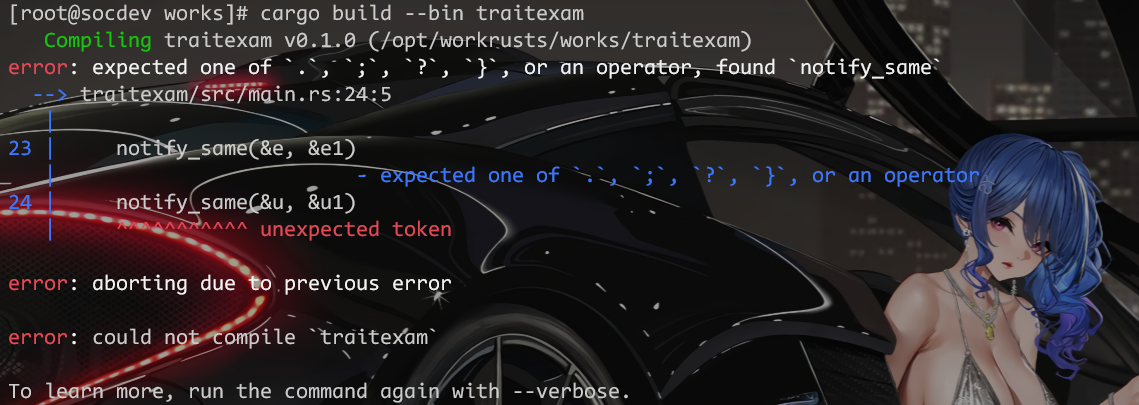
\includegraphics[scale=0.4]{rust_trait_bound.png}
  \caption{不同的Trait bound}
  \label{fig:rust_trait_bound}
\end{figure}

和Java/Golang一样,Rust也允许同一个类型实现多个Trait。同样的,多个Trait也可以作为
函数的参数进行传递:
\begin{code-block}{rust}
pub fn notify_multi_trait(item: &(impl Summary + Display)) {
    println!("{}", item);
    item.work();
}

// 也可以使用Trait bound
pub fn notify<T: (Summary + Display)>(item: T) {
    println!("{}", item);
    item.work();
}
\end{code-block}

如果函数接收多个参数,但这些参数都是多个trait组合的实现类型,就会导致函数签名特别
长,比如下方:
\begin{code-block}{rust}
fn some_function<T: Display + Clone, U: Clone + Debug>(t: T, u: U) -> i32 {
    ...
}
\end{code-block}
针对这种情况,就完全可以使用where模式进行简写:
\begin{code-block}{rust}
pub fn multi<T, U>(t: T, u: U) -> u8
where
    T: Summary + Display,
    U: Summary,
{
    ...
}
\end{code-block}

同样的,Trait也可作为函数/方法的返回值进行使用,如下:
\begin{code-block}{rust}
pub fn NewSummary() -> impl Summary {
    return User::create("zhangzz", 4, "zhangzz@outlook.com", true);
}
\end{code-block}
上述函数只能返回一个类型。如果需要返回不同的类型,我们编写的代码可能如下:
\begin{code-block}{rust}
pub fn NewSummary(swith: bool) -> impl Summary {
    if swith {
        return User::create("zhangzz", 4, "zhangzz@outlook.com", true);
    } else {
        return Empty{}
    }
}
\end{code-block}
很不幸的是,上述代码错误的,错误信息如下:
\begin{figure}[H]
  \centering
  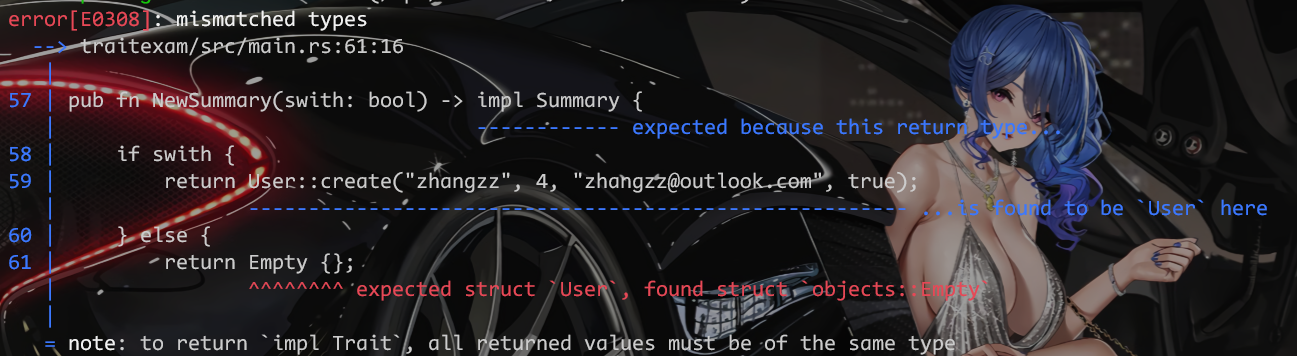
\includegraphics[scale=0.4]{rust_trait_return.png}
  \caption{试图返回不同的Trait实现类型}
  \label{fig:rust_trait_return}
\end{figure}
而这种需求的实现,则需要另外的方式进行实现。
